\begin{figure}
  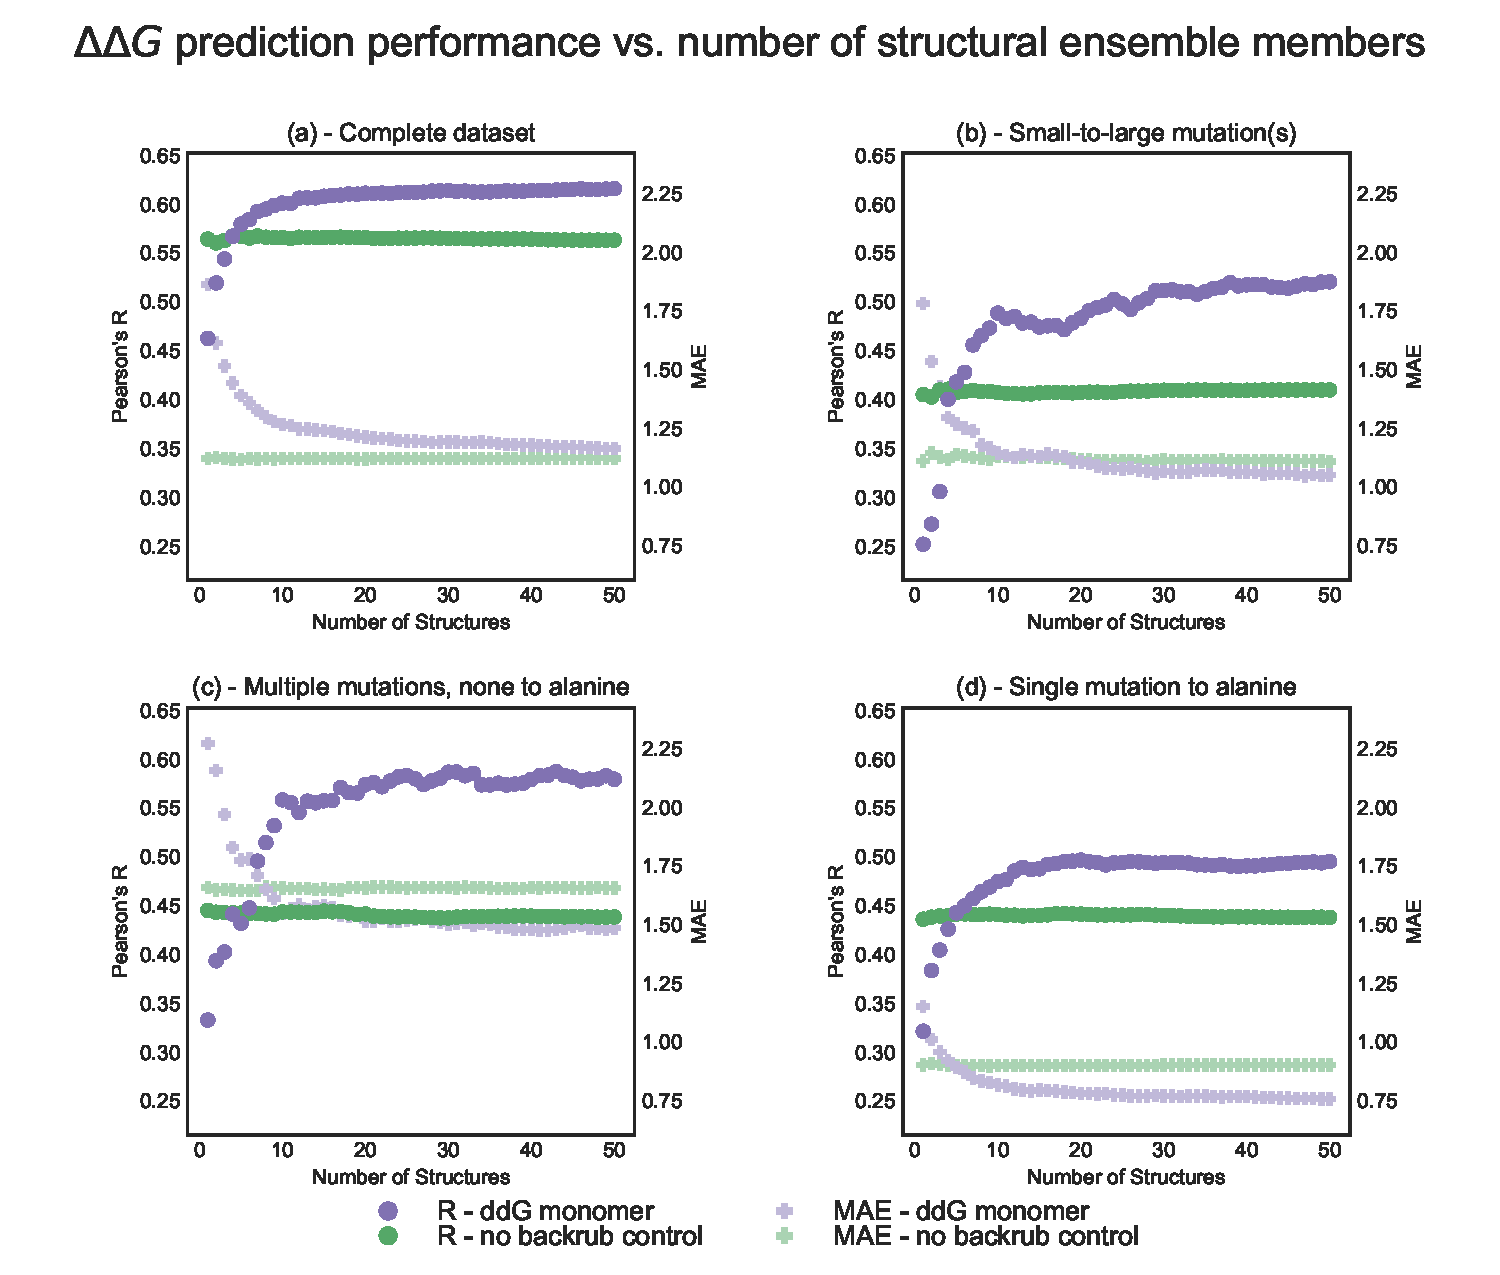
\includegraphics[width=\textwidth,keepaspectratio]{structs-v-corr-id-ddg-monomer-16-003-zemu-2.pdf}
  \caption[]{ % Old short caption: Flex ddG performance vs. number of averaged structures for ddG monomer
    Correlation (Pearson's R, left y-axis) and MAE (Mean Absolute Error, right y-axis) vs. number of averaged structures (x-axis), on the complete ZEMu set, and subsets.
    Pearson's R is shown with circular points, and MAE with faded plus-shaped points.
    A selection of key data underlying this figure can be found in \cref{tab:structs-v-corr-id-ddg-monomer-16-003-zemu-2-underlying-data}.
    Structures are not sorted, and are randomly added to the ensemble. 
    (a) Complete dataset (n = 1240)
    (b) Small-to-large mutation(s) (n = 130)
    (c) Multiple mutations, none to alanine (n = 45)
    (d) Single mutation to alanine (n = 748)
  } \label{fig:structs-v-corr-id-ddg-monomer-16-003-zemu-2}
\end{figure}
